\section{Background}

The sector of agriculture is one of the most important sectors for the Indian economy. The agricultural sector contributes about 20-25\% to the GDP of India. There has been a steady decline in the contribution of the agricultural sector to the Indian economy. This can be interpreted as a result of lack of research and development in this area. Especially in India agricultural sector has the least amount of growth and development compared to the other sectors which are actively implementing and adopting the cutting-edge technologies for rapid development. The introduction of Artificial intelligence seem to be the slowest in the agricultural sector compared to its explosive growth in other industries. This leaves the agricultural sector with a huge gap to incorporate and adopt the cutting-edge Artificial Intelligence and Machine Learning techniques for further improvement. This motivates us to research and develop AI and ML based solutions to solve the common problems in the agricultural sector. Even though there has been a considerable amount of research to introduce Artificial intelligence techniques into agriculture this project keeps the accessibility of the research and development as its top priority. 


\

Through the previous economic surveys the loss of income due to plat diseases and pests is about 20-25\%, which is a significant figure over the total economy of the agriculture. The areas of Artificial Intelligence and Machine Learning have seen an explosive development in the past few years. With the latest advancements in computer vision and natural language processing it is possible to device solutions to minimize the costs due to plant diseases and pests in agriculture. Most of the research done to incorporate these techniques never was really adopted and applied in the real world conditions. All these circumstances and conditions form the basis for this project. As most of the solutions that can be incorporated from the areas of Artificial Intelligence and Machine Learning are heavily dependant on the amount and quality of data, it is essential to improve the data resources and repositories to enable further research and development. It is very essential to analyze the available resources and weigh their pros, cons and biases to build robust production ready systems that are ready for use in fields. The study hypothesizes that it is possible to develop a solution accessible through widely available hardware to detect diseases in plants early and provide suitable solutions to counter the progression of that disease.


\section{Problem Addressed}

The project aims to introduce various Artificial Intelligence and Machine Learning techniques to the field of agriculture to minimize the losses due to pests and diseases. The study focuses on the detection and the possibility of early detection of various diseases in plants by using AI (Artificial Intelligence) and ML (Machine Learning). This study focuses on assessing the feasibility of making the developed solution available to regular people with minimal resources.

\

The study explores the feasibility of various machine learning techniques such as Support Vector machines, DNNs (Deep Neural Networks, RNNs (Recurrent Neural Networks) and Transformers for solving the task.

\

the problem is to develop a solution for early detection and detection of diseases in plants with minimal requirements that are accessible by everyone by exploring a wide range of machine learning and deep learning techniques. Focus on the feasibility of the developed solutions to be applied easily by normal people.

\

The recent advancements in natural language processing through the use of Large Language Models(LLMs) opened new ways to efficiently manage knowledge and data. The project deals with the problem of guiding the user further based on a predefined knowledge to minimize the loss due to the disease.

\

The solutions built using the AI and ML techniques are known to be computationally expensive to deploy and scale. The project aims to optimize the deployment of the proposed solution over limited resources. The deployment architecture focuses of effective horizontal scaling for maximum accessibility to the masses. It is important that the solutions that are developed in the research are reaching the people to make some difference. 

\

The proposed solution should be able to pass the test that the internal testing team does to prove its viability. The developed solution should be satisfactory to the initial users to continue for the further development. The model should show reliable results on the real world data that it is exposed to during the testing in fields. The current testing focus is majorly on the Chilli Leaf Curl virus and the ability of the model to differentiate the infected plant from the healthy ones. 

\

As the solutions that are currently being explored and the ones that are going to be developed in the future are heavily dependant on the quality and availability of data for training, we aim to provide a critical review on the state of various datasets with emphasis on pros, cons and biases observed in each of them. The problems that arise when combining multiple datasets to make a bigger dataset should also be effectively explained for the future research and development.

\ 

The study aims to provide well-documented research on the performance of a wide range of AI and ML techniques to detect diseases in plants. The project also focuses on the development of a mobile app that can be used to implement these modes on edge with a focus on accessibility on consumer hardware.


\section{Motivation}

\begin{center}
    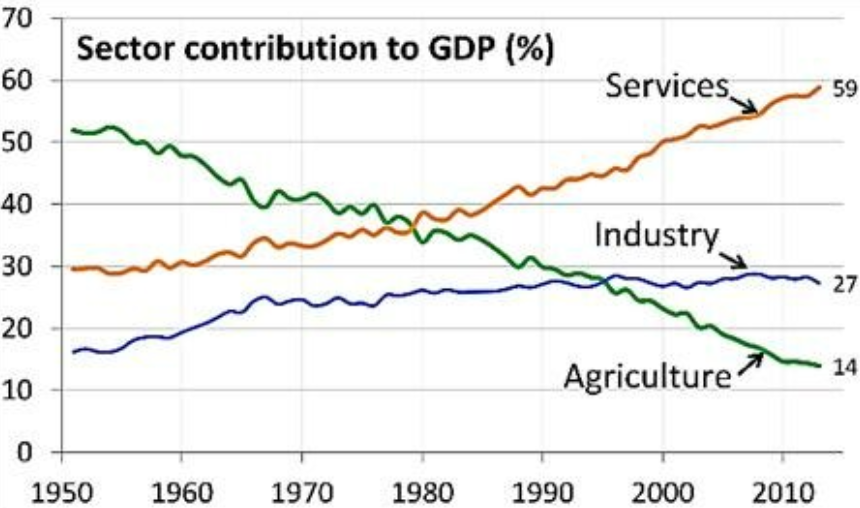
\includegraphics[scale=0.4]{decline_in_agriculture.png}\\
\end{center}



The occupations based on agriculture are becoming harder to sustain due to the environmental changes and unexpected changes in the climate. The field of agriculture has seen less growth and development compared to the other sectors mainly through the explosive development on Artificial Intelligence and Machine Learning techniques. The introduction of these latest techniques have been slow in the areas of agriculture compared to other sectors. We aim to contribute to the sector of agriculture by exploring some of the possible solutions to diagnose plat diseases and pests to minimize the losses to the farmers.

\

We believe that the research gets value when solutions are engineered based on the research. This project aims to analyze the complexities and optimizations in the deployment of the developed solutions. We are motivated by the fact that the knowledge is only useful when it is applied at the right place and the right time. The project aims to enable the users to get the required knowledge about the plant diseases and pests in the right time.

\

It is important to facilitate the future research and development through a critical review of the datasets that are used in the project based on their quality and document the challenges faced during the usage of these datasets. 

\

The project progresses on the motivation to introduce the latest Artificial Intelligence and Machine Learning techniques to the field of agriculture to improve the overall conditions of the sector.

\section{Scope of the Study/Project}   
The study starts small with a focus on the leaf curl virus and aims to generalize the solution to various common diseases in plants. The project focuses on the edge deployment of the solution on consumer hardware and these aspects set apart the current project from others.

 Define the boundaries and focus of the project.
Specify what is included and excluded.
Highlight the target domain, dataset, or systems under consideration.

Conclude by discussing the organization of the project report. Briefly describe what each chapter covers.
Ensure the flow is logical and coherent.

